\documentclass[tikz,border=2pt]{standalone}
\usepackage{amsmath,amssymb}
\usepackage{tikz}
\usetikzlibrary{arrows.meta}

\begin{document}
% The extended real line adds two symbols at the ends: -∞ < x < +∞ for every real x.
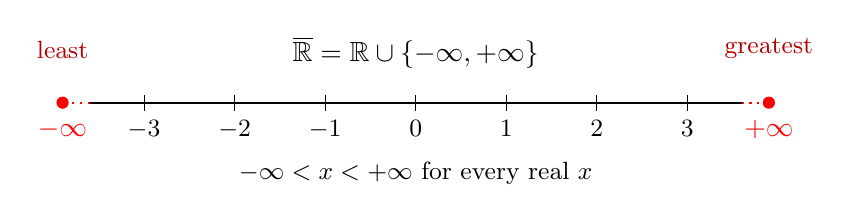
\begin{tikzpicture}[x=1.15cm]
	\draw[thick] (-3.6,0) -- (3.6,0);
	\foreach \x in {-3,-2,-1,0,1,2,3} {\draw (\x,0.1) -- (\x,-0.1); \node[below=3pt, font=\small] at (\x,0) {$\x$};}
	\fill[red] (-3.9,0) circle (2.2pt);
	\fill[red] (3.9,0) circle (2.2pt);
	\node[red, below=3pt] at (-3.9,0) {$-\infty$};
	\node[red, below=3pt] at (3.9,0) {$+\infty$};
	\draw[red, dotted, thick] (-3.6,0) -- (-3.9,0);
	\draw[red, dotted, thick] (3.6,0) -- (3.9,0);
	\node[above=6pt] at (0,0.1) {$\overline{\mathbb{R}}=\mathbb{R}\cup\{-\infty,+\infty\}$};
	\node[red!70!black, above=4pt, font=\small] at (-3.9,0.3) {least};
	\node[red!70!black, above=4pt, font=\small] at (3.9,0.3) {greatest};
	\node[below=18pt, font=\small] at (0,0) {$-\infty<x<+\infty$ for every real $x$};
\end{tikzpicture}
\end{document}
